\chapter{Basics}
In this section the basic concepts and terms needed for further discussion will be introduced. This includes general machine learning terminology and how it applies to Sparked, as well as terminology of Sparked that bases on these fundamentals. It is important to note, that Sparked itself does not contain any machine learning capabilities. All machine learning evaluation comes from CODA. Because of that the terminology will generally be adopted from CODA, which has its roots in supervised learning, specifically classification. 

Supervised learning tries to approximate a function from a datapoint to a value by learning the underlying rules from data, where the corresponding value is already known. There are two types values, discrete ones, labels like spam or no spam. Problems that fall in this category are called classification problems. The other having continuous values, called regression problems, like a good price for a used car. In the context of sparked, supervised learning problems will not be differentiated as classification or regression problems. All problems will be defined by four values, dataset, classifier, validation method and evaluation metric.
To learn the labeling rules supervised learning algorithms need a dataset that has already been labeled. Within the context of Sparked, a dataset is the data from which the program is supposed to learn the underlying rules from. 

The underlying algorithm to evaluate the dataset with, is the classifier. Since Sparked does not differentiate between classification and regression problems, such an algorithm may be a classification or regression algorithm even though the name might suggest the former. Classifiers may have additional information attached, hyperparameters the classifier needs to further adjust it to the giving problem. These hyperparameters have a special place in machine learning, because they are typically a fixed value set at the start of evaluation and not learned or adjusted from the ML program. Optimizing these hyperparameters is a major concern in machine learning problems and automating this optimization one of the main goals of automated machine learning projects like CODA.
Part of training is validating the output. In its essence that means taking a part of the dataset and use it not for training but have the algorithm predict the known label after training and checking how good the predictions where. This is helpful not only to put a number on how good the training was and helps discover cases of overfitting, that are always a concern with supervised learning. Since the dataset is partially not used for validation, it does reduce the number of datapoints the program has to train. There are several ways to address this problem, getting the right balance between validation and training. These must be supplied in the validation method.

An important part of evaluating how good a training was, is to define what good means. For credit card fraud data, where almost all transactions are non-fraudulent it is not enough to measure the accuracy or how many predictions where correct, as just predicting all of them as good would be incredibly accurate, but not give any valuable information whatsoever. The measure to apply must be supplied by the user and is called the metric or target metric within Sparked. 
Combining these four values, dataset, classifier with hyperparameters, validation method and metric is the information Sparked needs to start an evaluation with CODA. Such an evaluable set will be called task. 

The focus of this software is however not to solve machine learning problems or tasks, but to compare multiple task against each other, that only differ in the classifier, either its algorithm or its hyperparameters. Such a set of tasks will be called an order. The order is the main object in Sparked. All actions will be done on an Order. 

\section{State of the art}
There are several interesting projects when it comes to visual interfaces for machine learning software. One of these is the web application OpenML. OpenML [\hyperlink{www.openml.org}{www.openml.org}] or open machine learning gives access to machine learning tools to a broad audience, including readily available datasets and predefined classification algorithms.\\
The general look and feel of OpenML is very bright with strong vivid colors and hard corners. Separate values are often put right next to each other, only separated by a dash. This gives the UI a fresh and tidy look and allows a lot of information to be put on a small amount of space, but it also makes it hard to identify entries at a glance. The lists are not paged and can show all results at the same time, using on the fly loading of additional items while scrolling. While this should make it very hard to find any data, the usage of filters and search bars helps find entries fast. \\
Very notable is the usage of likes, reach and impact values, giving the page a social media vibe. This is part of the core idea of OpenML, to facilitate sharing and reuse of machine learning tools, but has no correspondent feature in Sparked. 
 
\begin{figure}
	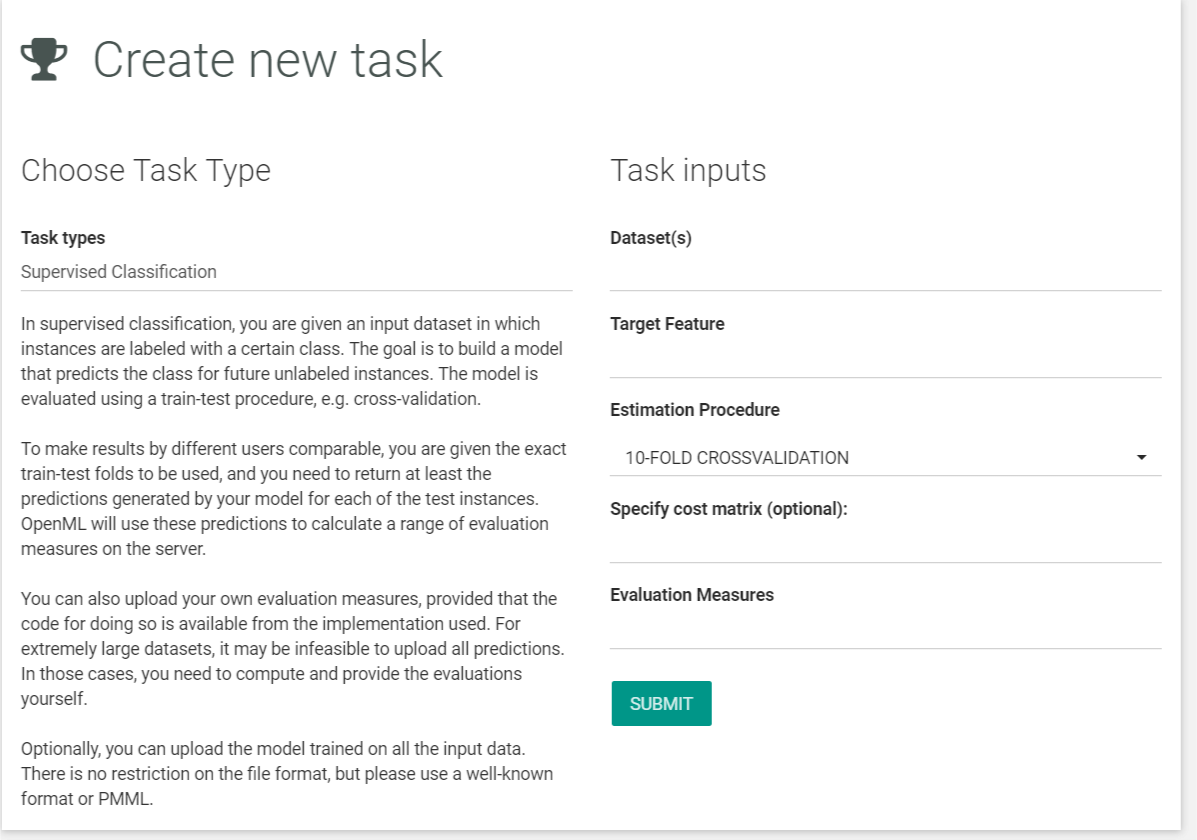
\includegraphics[width=\textwidth]{openML-Task.png}
	\caption{OpenML UI, clean and colorful with a lot of tight packed information. The basic features of OpenML allow the creation of tasks. }
\end{figure}

\begin{figure}
	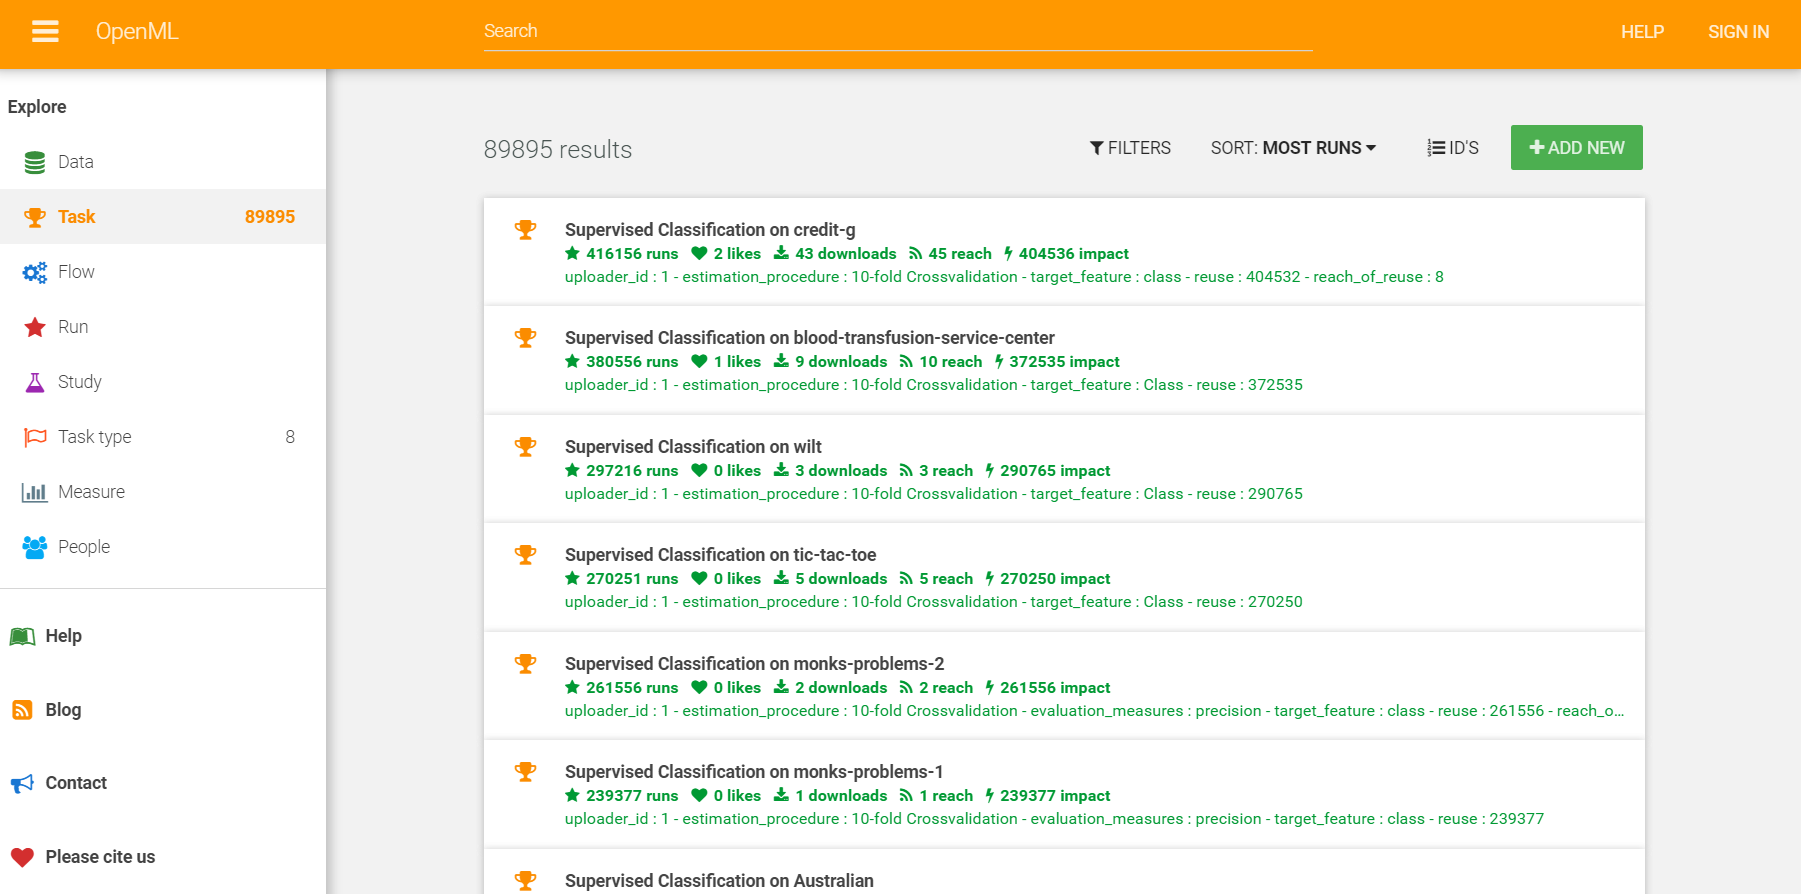
\includegraphics[width=\textwidth]{openML-BaseDesign.png}
	\caption{Task Creation in AutoML requests most of the data an order creation in Sparked will need. }
\end{figure}

While creating a task, the user will choose what kind of machine learning they want, like supervised learning, supervised regression and clustering, an estimation procedure which maps to the validation method in Coda and the evaluation measures. All these input steps are situated on the same view. As selected values stay visible, a overview over the selected data is available at all times.\\

Like Sparked, AutoML provides a view to see the evaluation measures. Here the concrete values are displayed as well as a graphical representation. Here AutoML does not differentiate between the measures and shows all of them on one site with help of the JavaScript chart library highcharts. This sometimes led to performance issues in the browser, making the page appear sluggish, on some occasion even freeze. It should be kept in mind, that even good JavaScript chart libraries can have performance issues, especially while loading and scaling multiple charts at the same time.

\begin{figure}
	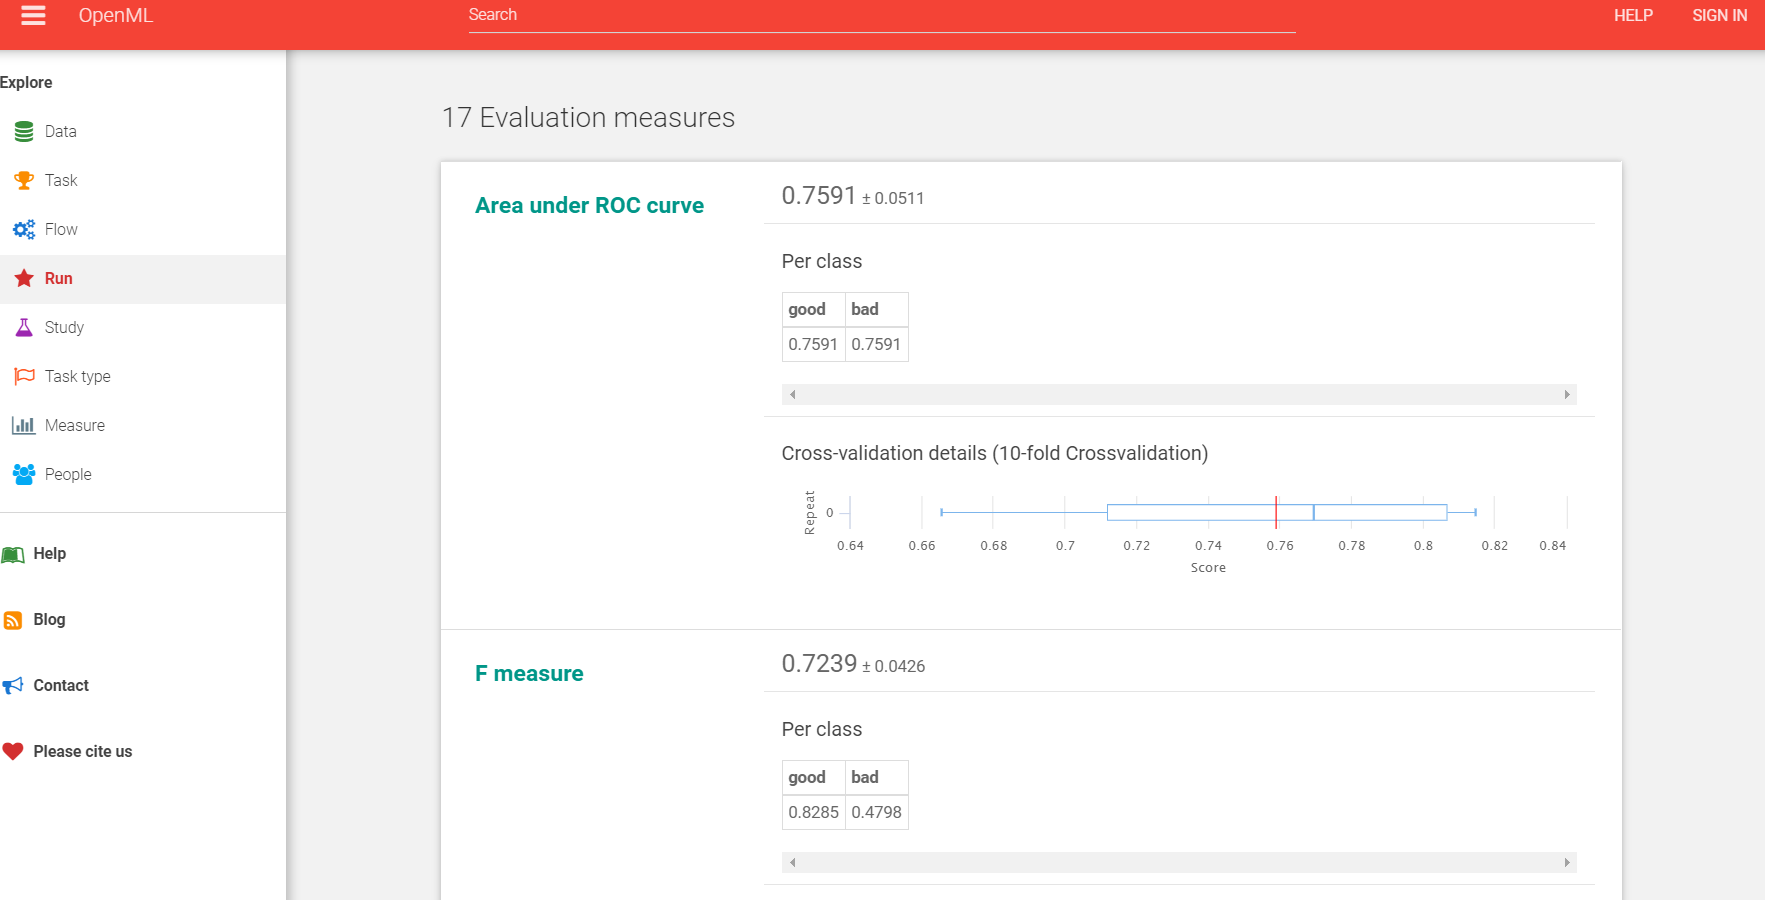
\includegraphics[width=\textwidth]{EvaluationMeasures.png}
	\caption{AutoML displays several evaluation measures at the same time with graphical components using Highsofts charting JavaScript library highcharts. }
\end{figure}
